\chapter{Fundamentação} \label{ch:fundamentation}

Este Capítulo apresenta toda a fundamentação necessária para o entendimento do trabalho. 
Ele é separado em duas Sessões, na primeira, são apresentados os conceitos básicos sobre 
o StarVZ e seu Workflow e, na segunda, discute-se sobre os trabalhos relacionados.

\section{Conceitos Básicos} \label{sect:basic-concepts}

O StarVZ \cite{ref:starvz} é um \emph{workflow} de análise de performance cujo objetivo é facilitar
a avaliação de aplicações \emph{task-based}. Ele é composto de duas fases, cada uma delas sendo uma 
combinação de diversas ferramentas, que resultam em um \emph{framework} rápido, consistente, flexível 
e versátil. Seu objetivo é auxiliar na análise de performance e na verificação de hipóteses de aplicações 
executadas sobre ambientes heterogêneos.

A primeira fase, que pode ser visualizada na Figura \ref{fig:starvz-workflow1}, consiste em uma etapa de pré-processamento.
Nela, os dados são limpos, ordenados e filtrados, combinando entradas de diferentes fontes para a criação de novas informações.
Essa fase é muito custosa do ponto de vista computacional, pois as entradas podem ser grandes. Isso pode ser um problema em 
determinadas situações pois, por exemplo, para processar uma entrada de aproximadamente 18GB, uma máquina equipada com um Intel(R)
Xeon(R) CPU E3-1225 v3 @3.20GHz e 32GB de memória principal levou em torno de 32 minutos para finalizar o processamento.

\begin{figure}[H]
 \centerline{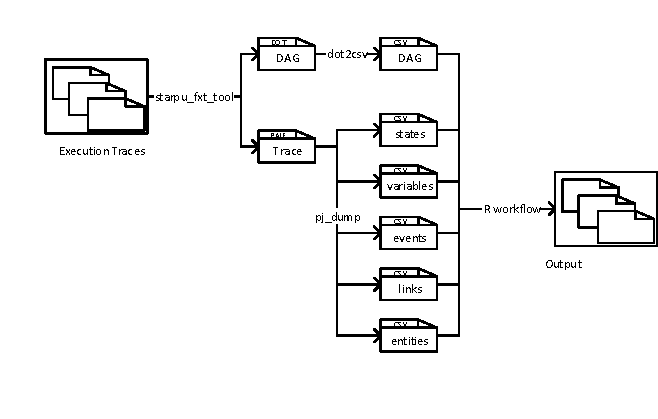
\includegraphics[width=1\textwidth]{./img/step1-final.pdf}}
 \caption{Passos de processamento do StarVZ}
 \label{fig:starvz-steps}
\end{figure}

\section{Trabalhos Relacionados}\label{sect:related-work}